\documentclass[11pt]{article}

\usepackage{graphicx}
\usepackage{hyperref}
\usepackage{natbib}
\usepackage{amsmath}

\bibliographystyle{plain}
\setlength{\textwidth}{6.5in}
\setlength{\headheight}{0in}
\setlength{\textheight}{8.0in}
\setlength{\hoffset}{0in}
\setlength{\voffset}{0in}
\setlength{\oddsidemargin}{0in}
\setlength{\evensidemargin}{0in}


\title{Computational Physics -  Problem Set 7}
  
\author{Frederik Holst Knudsen}


\begin{document}

\maketitle
Github URL: https://github.com/frederikholst/phys-ga2000
\section{Newman 6.16}
Assuming circular orbits, the forces acting on the satellite is:
$$F_{Total}=F_{Earth}+F_{Moon} + F_{centrifugal}=0$$
$$F_{Total}=\frac{GM}{r^2}-\frac{Gm}{(R-r)^2}-\frac{v^2}{r}=0$$
With $\omega =\frac{v}{r}$:

$$F_{Total}=\frac{GM}{r^2}-\frac{Gm}{(R-r)^2}=\omega^2r $$
The gravitational force between M and m provides the centripetal force needed to maintain the orbit. This gives:

$$\omega^2=\frac{GM}{R^3}$$
And we have:
$$\frac{M}{r^2}-\frac{m}{(R-r)^2}=\frac{Mr}{R^3} $$

To rescale the equation, we let $m'=m/M$ and $r'=r/R$:

$$\frac{M}{(r'R)^2}-\frac{m'M}{(R-r'R)^2}=\frac{Mr'R}{R^3} $$

Dividing through with $M/R^2$ gives:
$$\frac{1}{r'^2}-\frac{m'}{(1-r')^2}=r' $$

By iteratively updating r using the Newton's method, the lagrange point is found to be 326 million kilometers with 0.8 as the initial guess for r' and with a tolerance of $1\times 10^{-15}$. Strangely, this is still off by a significant amount as compared to the actual value of 323 million kilometers. 

Similarly, the lagrange points for Earth and Sun is 148.10 million kilometers from the sun, and finally the lagrange point between a Jupiter-mass planet orbiting the Sun at the distance of the Earth is at 139.625 million kilometers from the sun. 

\section{Brent's 1D minimization Method}:

We now implement Brent's minimization method by having three different ways of performing the iterative steps towards the minimum. The three differnet methods are the secant method, which is used if point b and c are sufficiently far apart, the parabolar method which is used if the next step falls within the range of point a and c, and finally the bisection method is used if the two others fail. See the problem2.py for detailed breakdown of the function. The minimum of the function $y(x)=(x-0.3)^3*e^{x}$ is found to be 0.2999528 which is within machine precision (8.42218566e-07) of the actual value found using SciPy minimization. 
\end{document}


\begin{figure}[!htbp]
    \centering
    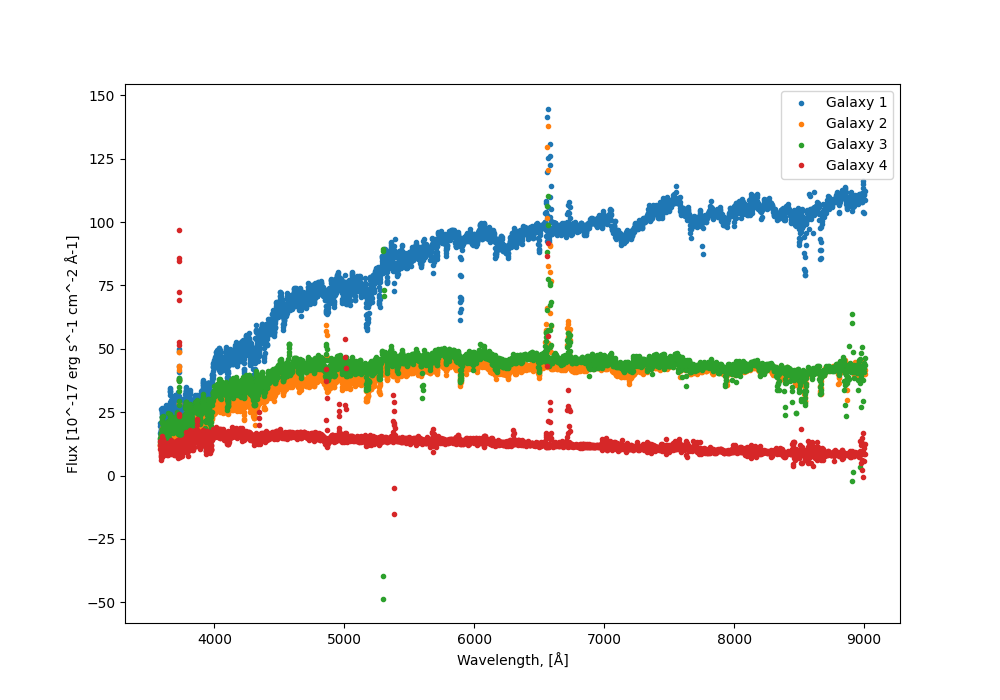
\includegraphics[width=0.7\textwidth]{Galaxies.png}
    \caption{The spectra of the first five galaxies are seen plotted against wavelength.}
    \label{Balmer}
\end{figure}
